\chapter{Conclusion}
\label{conclusion}

After being sought for many years at different collider experiments, the Higgs boson was discovered by the ATLAS and CMS experiments in 2012, confirming the leading theory for the source of electroweak symmetry breaking and filling in the last missing piece of the Standard Model. After its discovery, measurements of the particle's detailed properties and searches for new particles decaying to Higgs final states were both extremely important in constraining physics beyond the Standard Model. This dissertation presented this evolution through two results: the observation and measurement of the Higgs boson in the \HWWfull channel at $\sqrt{s} = 7 \TeV$ and $\sqrt{s} = 8 \TeV$ and a search for Higgs pair production in the $HH\to b\bar{b}b\bar{b}$ channel at $\sqrt{s} = 13 \TeV$ with the ATLAS detector in $pp$ collisions at the Large Hadron Collider.

In the \HWWfull, results from both the discovery of the Higgs boson and the full ATLAS Run 1 dataset were presented. The Higgs boson was discovered with a $6.1\sigma$ significance in a combination of the $H\to\gamma\gamma$, $H\to ZZ 4\ell$, \HWWfull with $4.2\ifb$ at $\sqrt{s} = 7 \TeV$ and $5.2\ifb$ at $\sqrt{s} = 8 \TeV$. With the full $20.3\ifb$ at $\sqrt{s} =  8 \TeV$ and $4.2\ifb$ at $\sqrt{s} = 7 \TeV$, ATLAS achieved discovery level significance in the $\HWW$ channel alone and obtained the first observation of vector boson fusion production in that channel. The combined signal strength is measured to be $\mu = 1.09^{+0.23}_{-0.21}$. The total observed significance of the $\HWW$ process is observed to be $6.1\sigma$ (with $5.8 \sigma$ expected). Advanced methods for background reduction and estimation, particularly in same-flavor lepton final states, are shown. The VBF signal strength is measured to be $\mu_{\rm VBF} = 1.27^{+0.53}_{-0.45}$ with an observed significance of $3.2\sigma$ (with $2.7 \sigma$ expected). 

These results required many novel innovations. The increase of pileup interactions in the higher instantaneous luminosity LHC conditions of 2012 led to a degradation of missing transverse momentum resolution. As a result, the prominent $\ZDY$+jets background of the same flavor \HWWfull final states increased greatly. New variables, including a track-based missing transverse momentum and a measurement of the balance between the dilepton system and recoiling jets, allowed for significant reduction of this background. In the VBF channel, selections were optimized to exploit the unique VBF final state topology. Incorporating these variables into a boosted decision tree technique allowed the analysis to exceed the $3\sigma$ observation threshold.

After the end of Run 1, the results of Higgs measurements from ATLAS were combined with those from CMS to produce the most precise measurements of the Higgs boson so far~\cite{ATLASCMSHiggs}. Figure~\ref{fig:ATLAS-CMS-comb} shows the combination of ATLAS and CMS data for the Higgs signal strength in and coupling measurements. In the signal strength measurements of gluon fusion and vector boson fusion, the $\HWW$ channel provides the tightest constraints. Additionally, the Higgs coupling to $W$ bosons is the most precisely measured with a relative uncertainty of $10\%$. 

\begin{figure}[h!]
  %\vspace{20pt}
  \centering
  \captionsetup{justification=centering}

   \begin{subfigure}[t]{0.5\textwidth}
        \centering
        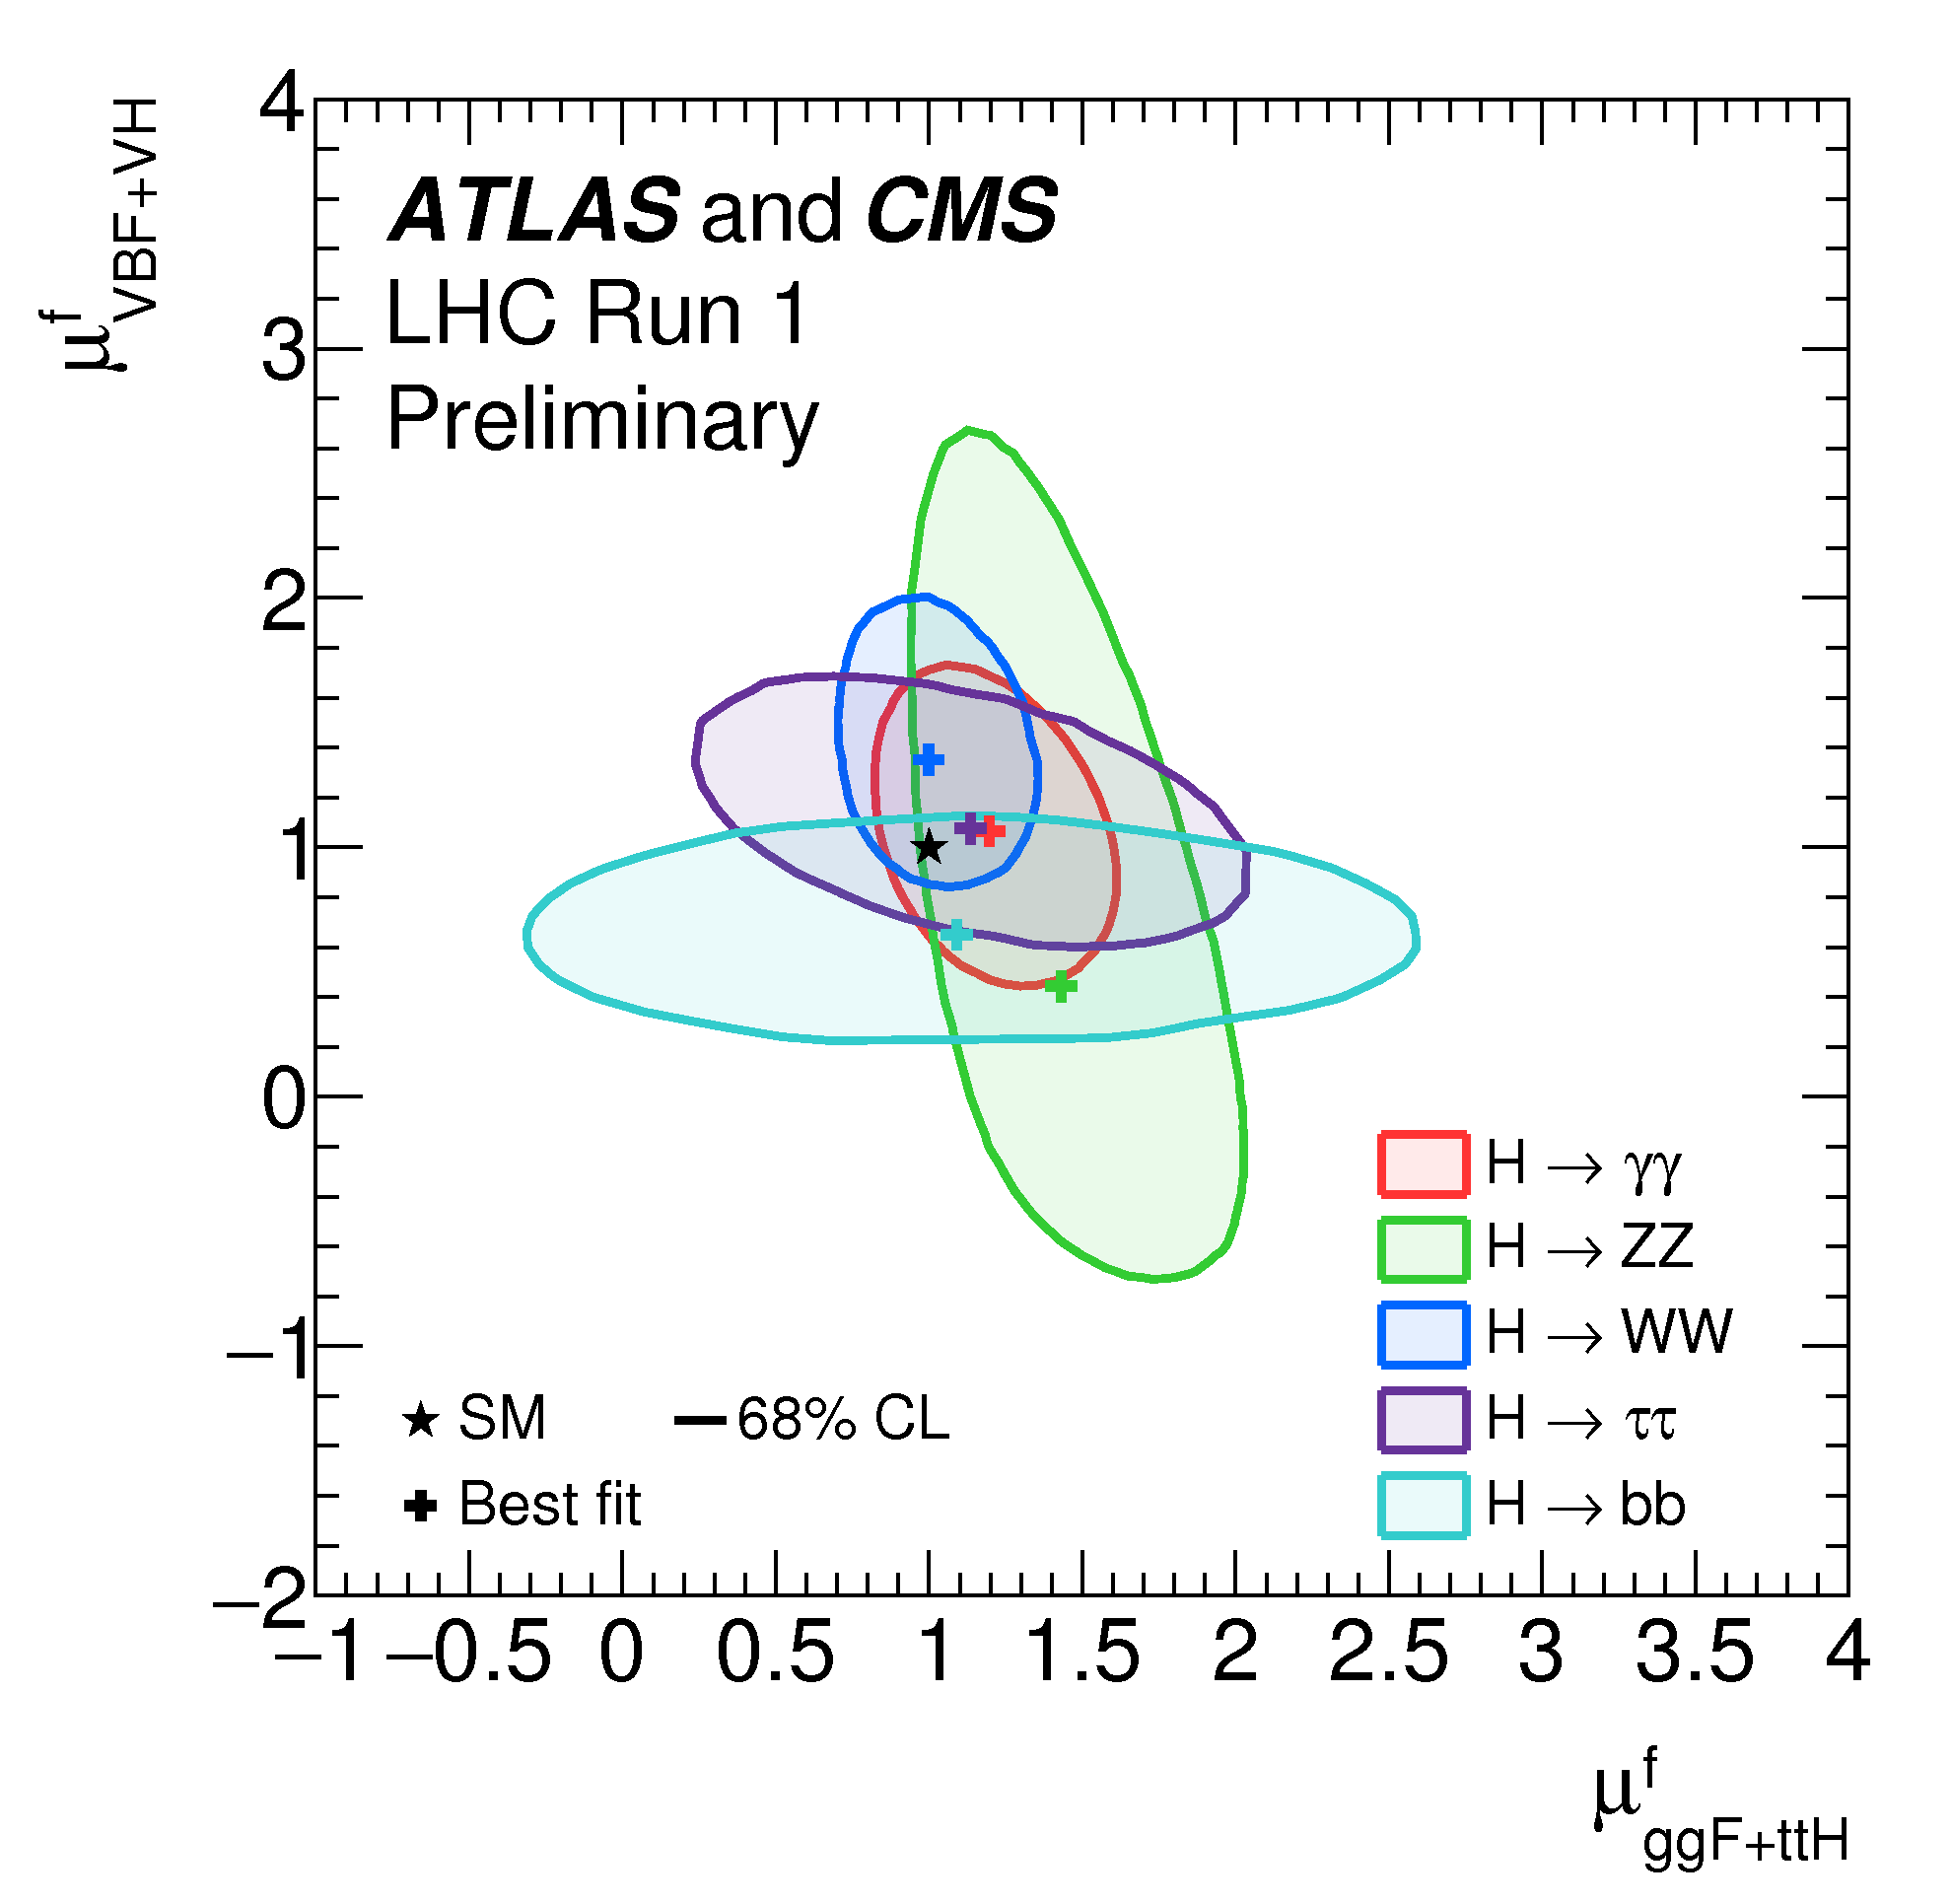
\includegraphics[width=\textwidth]{figures/ATLAS_CMS_mu}
        \caption{}
    \end{subfigure}%
    \begin{subfigure}[t]{0.5\textwidth}
        \centering
        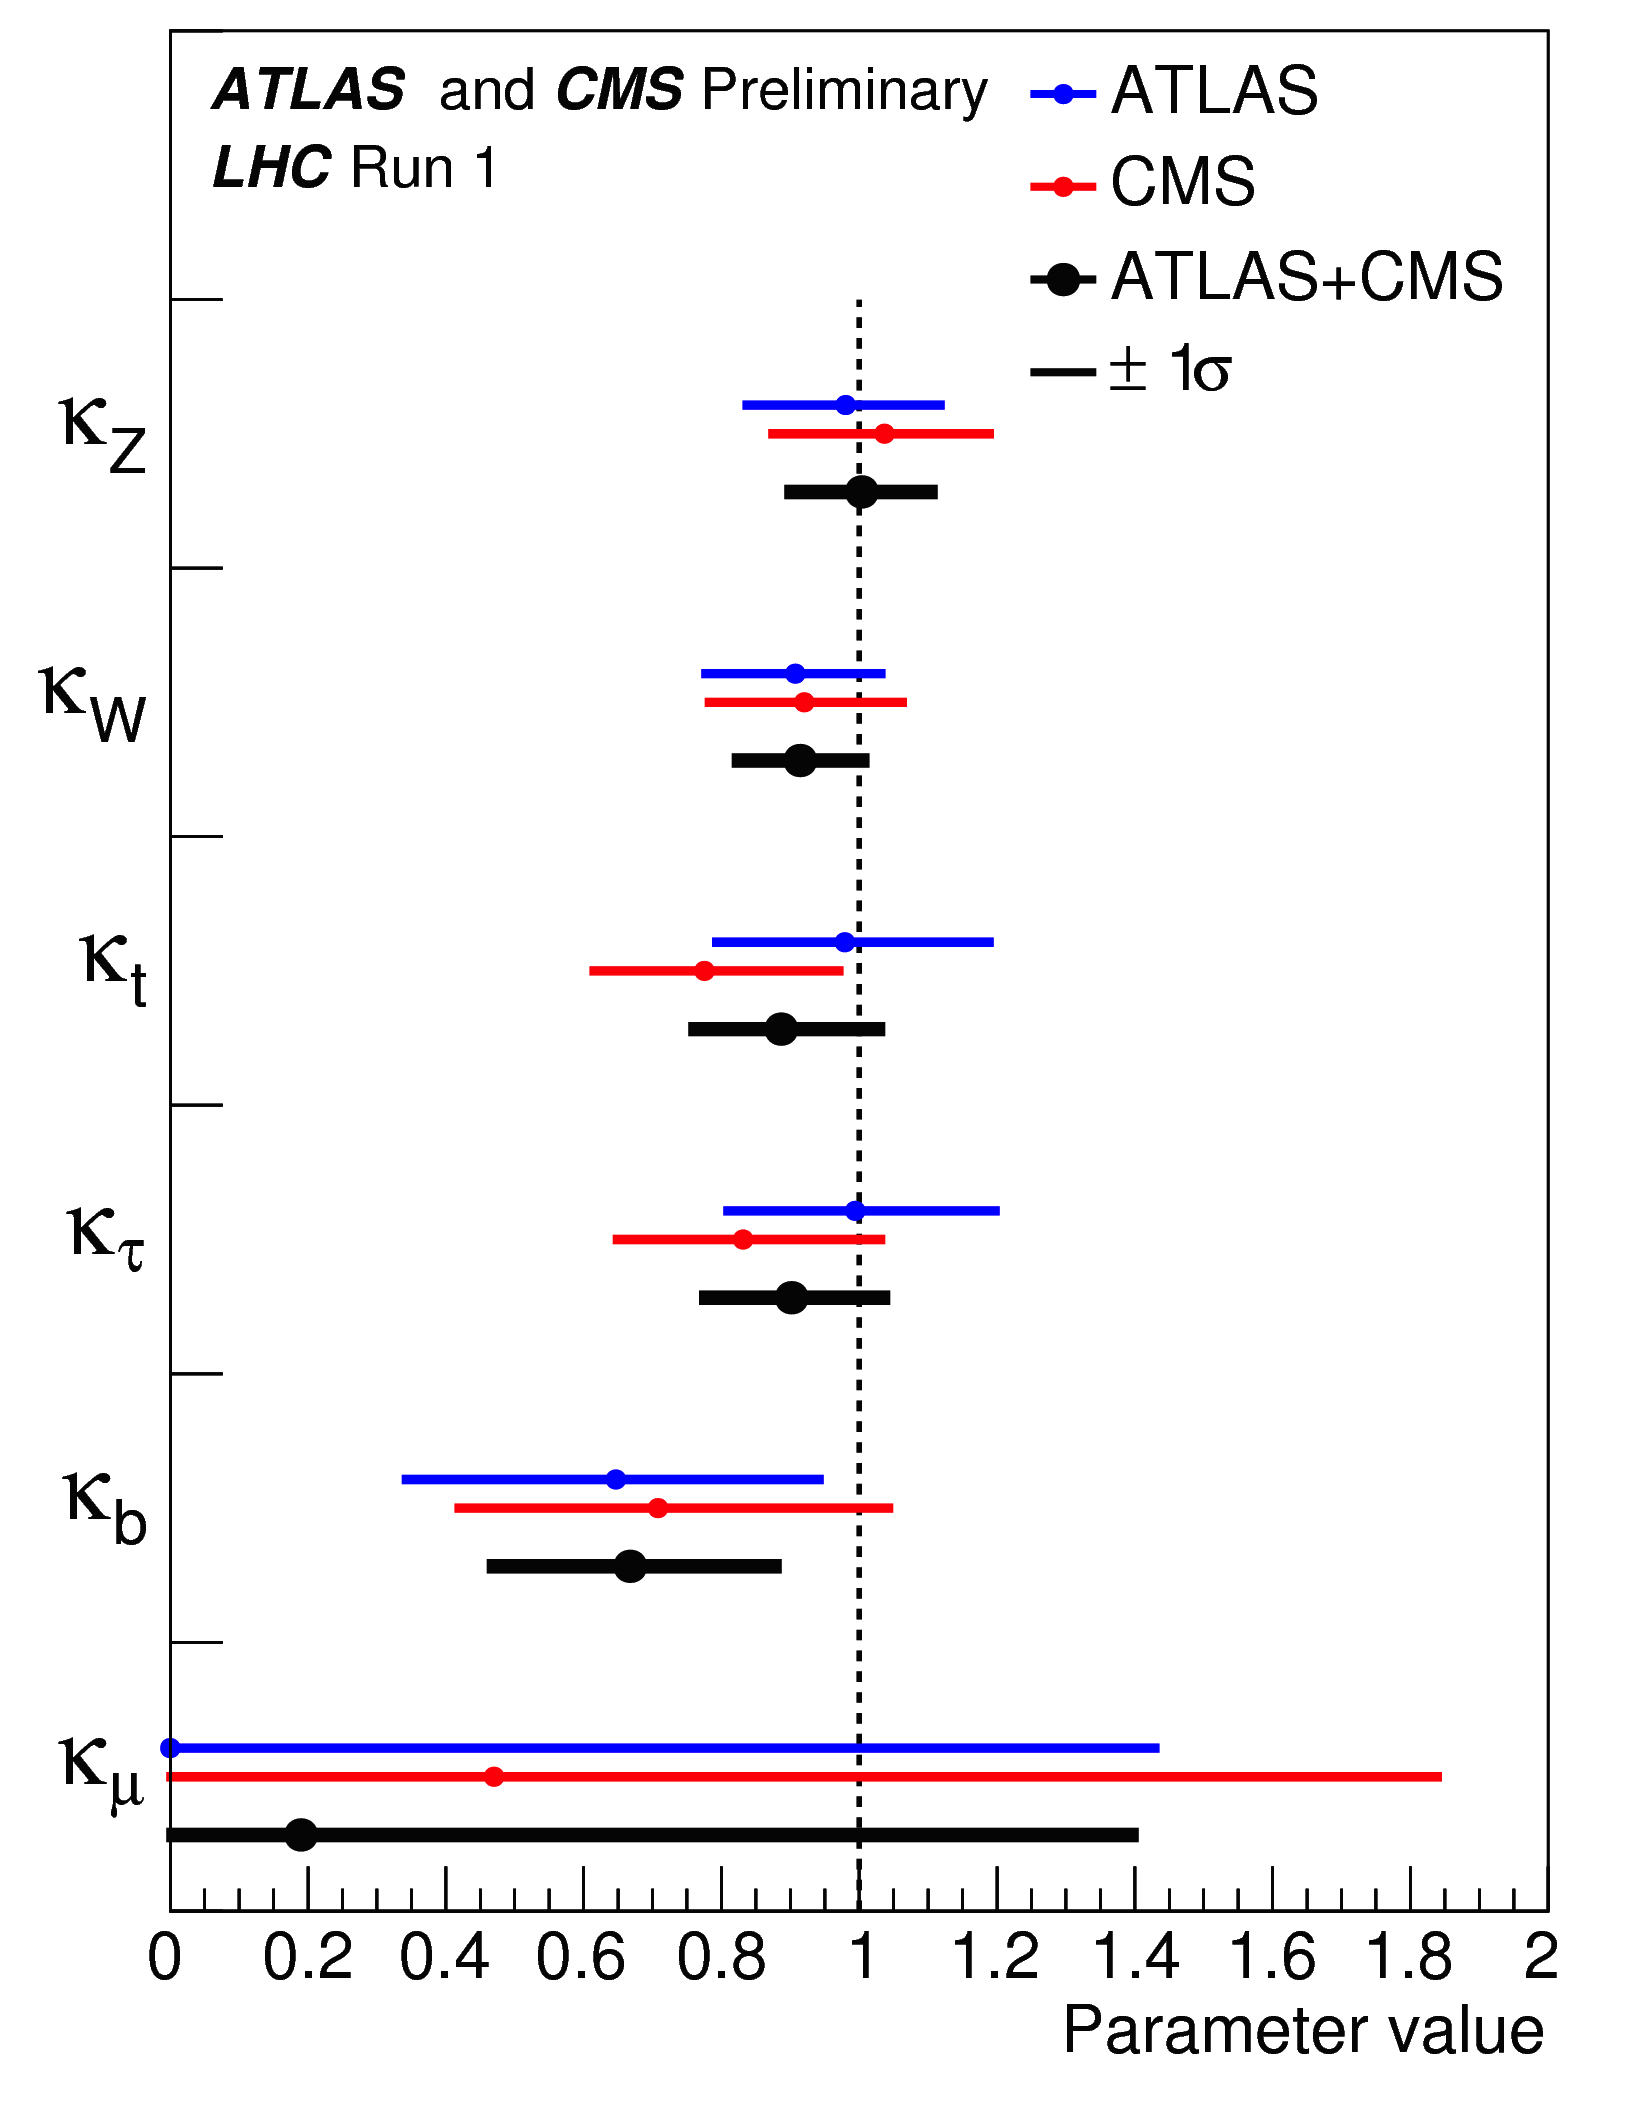
\includegraphics[width=\textwidth]{figures/ATLAS_CMS_couplings}
        \caption{}
    \end{subfigure}

   \caption{Combined ATLAS and CMS measurements in Run 1 for (a) Higgs signal strength in gluon fusion and VBF and (b) Higgs couplings normalized to their SM predictions}
  \label{fig:ATLAS-CMS-comb}
\end{figure}

With the discovery of the Higgs firmly established and its properties measured, a natural next step was to search for new physics with Higgs final states. At $\sqrt{s} = 13 \TeV$, a search for Higgs pair production in the $b\bar{b}b\bar{b}$ final state with $3.2\ifb$ was conducted. A signal region optimized for the boosted final states arising from high mass resonances was constructed. This signal region utilized large-radius calorimeter jets and $b$-tagging with small radius track jets to maximize the signal acceptance. No significant excesses were observed, and upper limits on cross sections are placed for spin-2 Randall Sundrum gravitons (RSG) and narrow spin-0 resonances. The increase in center of mass energy in Run 2 allowed this analysis to extend upper limits up to $3 \TeV$, while previous results from ATLAS in Run 1 only quotes limits up to $2 \TeV$. The cross section of $\sigma(pp \to \Gkk \to hh \to b\bar{b}b\bar{b})$ with $k/\bar{M}_{\rm Pl}=1$ is constrained to be less than $70 \fb$ for masses in the range $600 < m_{\Gkk} < 3000 \GeV$. For the RSG model with $k/\bar{M}_{\rm Pl}=2$, cross sections limits between $40\fb$ and $200 \fb$ are set for the mass range of $500 < m_{\Gkk} < 3000 \GeV$. The cross section upper limits for $\sigma(pp \to H \to hh \to b\bar{b}b\bar{b})$ ranges from $30$ to $300 \fb$ in the mass range of $500 < m_{H} < 3000 \GeV$. 

While there has been a rigorous program of measurements and searches involving the Higgs, there is still much room for improvement at the High Luminosity LHC (HL-LHC) and beyond. The measured signal strength for VBF production in $\HWW$ still has a relative error at the level of $40\%$, largely dominated by statistical uncertainty. Projections for the HL-LHC show that the uncertainty on the VBF signal strength can be reduced to approximately $15\%$ with $3000 \ifb$~\cite{HiggsProj,ScopingDocument}. This uncertainty also assumes that theoretical uncertainties on the signal, which would be the largest contribution in this dataset, remain as they are now. Improvements in the theoretical understanding of the Higgs signal would also reduce the signal strength uncertainty dramatically. Such precision measurements allow for measurements of the Higgs coupling to vector bosons precise to the few percent level, therefore giving much power to constrain or discover new physics. 

The prospects for detection of resonant di-Higgs production at the HL-LHC are also quite promising. Figure~\ref{fig:HH_prospect} shows projections for the discovery significance of RSG signals at the HL-LHC in the $\FourBfull$ search~\cite{ScopingDocument}. In all detector budget scenarios, a $1.5 \TeV$ resonance is above or near $5\sigma$ significance, while a $2 \TeV$ resonance is between $4$-$5\sigma$ except for the lowest budget. 
%
\begin{figure}[h!]
  %\vspace{20pt}
  \centering
  \captionsetup{justification=centering}

  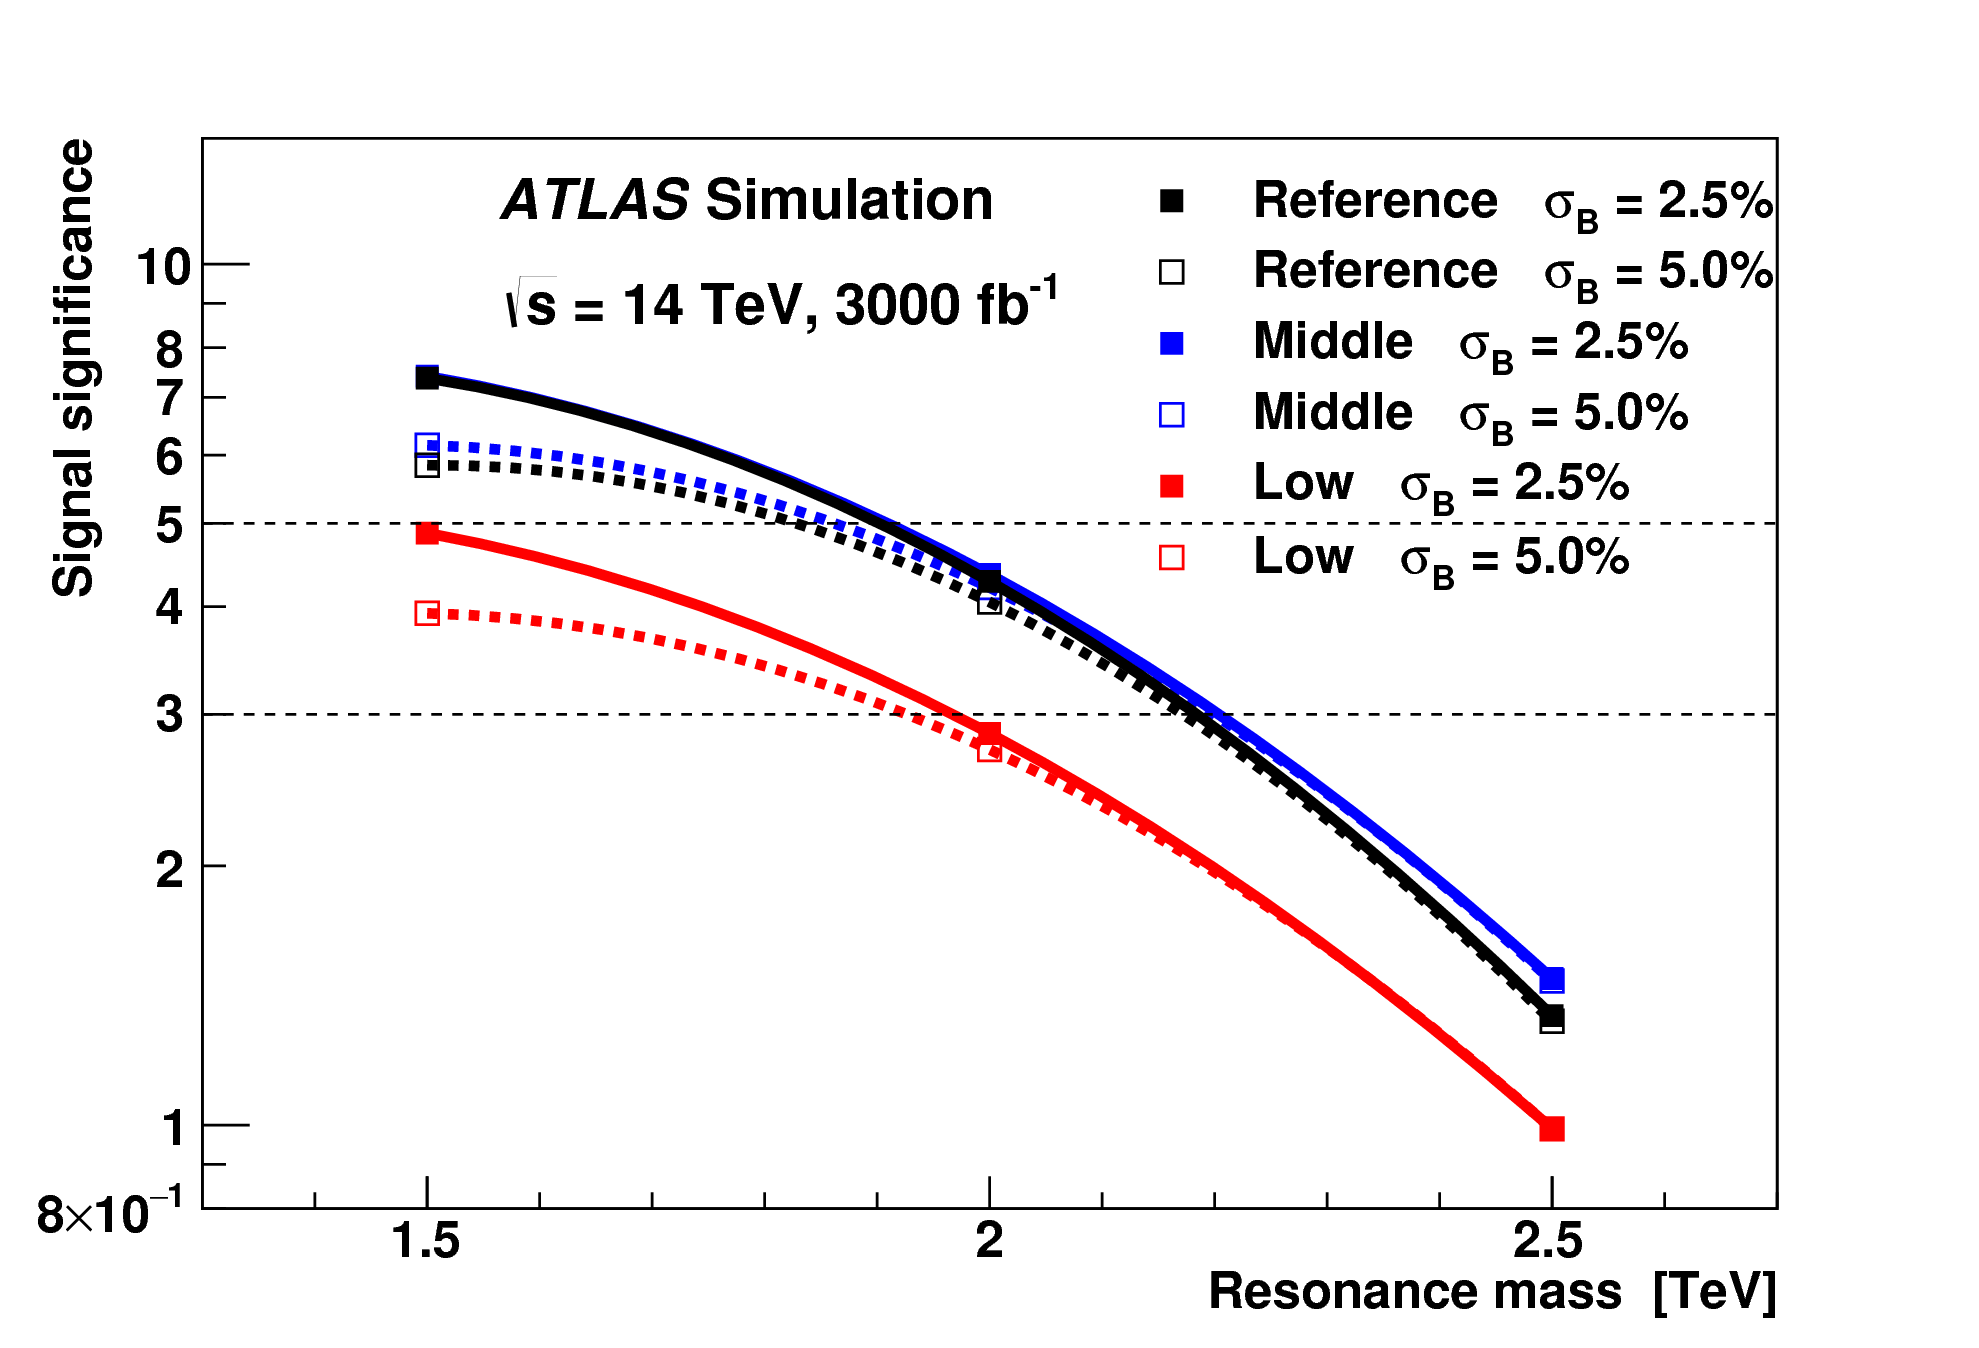
\includegraphics[width=0.6\textwidth]{figures/HH_scoping}
        
   \caption{Discovery significance for RSG models at the HL-LHC in three different budget scenarios~\cite{ScopingDocument}. Systematic uncertainties on the background prediction ($\sigma_B$) of $2.5\%$ and $5.0\%$ are both tested.}
  \label{fig:HH_prospect}
\end{figure}
%

The Higgs will continue to be an incredibly powerful tool in the understanding of nature at the HL-LHC and beyond. Through both precision measurements and searches, the nature of electroweak symmetry breaking will be better understood and the potential for the discovery of physics beyond the Standard Model has never been greater. 



